% Inbuilt themes in beamer
\documentclass{beamer}
\usepackage{tikz}
\usepackage{svg}
\usepackage{multimedia}
\usepackage{tcolorbox}

% Define a custom block
\newtcolorbox{blackblock}[1][]{
  colback=white,         % Background of body
  colframe=black,        % Border color
  coltitle=black,        % Title text color
  colbacktitle=white,    % Title background color
  fonttitle=\bfseries,   % Bold title font
  title=#1,              % Title text
  boxrule=1pt,         % Border width
  arc=1mm,               % Rounded corners (optional)
  left=1mm, right=1mm, top=1mm, bottom=1mm,
}
\newtcolorbox{redblock}[1][]{
  colback=white,         % Background of body
  colframe=red,        % Border color
  coltitle=red,        % Title text color
  colbacktitle=white,    % Title background color
  fonttitle=\bfseries,   % Bold title font
  title=#1,              % Title text
  boxrule=1pt,         % Border width
  arc=1mm,               % Rounded corners (optional)
  left=1mm, right=1mm, top=1mm, bottom=1mm,
}

% Theme choice:
\usetheme{kellentheme}

% Title page details: 
\title{Temporal Difference Flows \cite{farebrotherTemporalDifferenceFlows2025}} 
\author{Kellen Kanarios}
\date{\today}
\logo{
    % 
\includegraphics[width=0.05\linewidth]{figures/umich-m.png}
}


\setbeamertemplate{footline}[myfootline]
\begin{document}

% Title page frame
\begin{frame}
    \titlepage 
\end{frame}


\begin{frame}{Outline}
    \tableofcontents
\end{frame}

\section{Motivation}
\begin{frame}{Variational inference with normalizing flows \cite{rezendeVariationalInferenceNormalizing}} 
    \begin{itemize}
        \item Want to maximize log-likelihood \( \log p_{\theta}(\mathbf{x}) \). Introduce latent \( \mathbf{z} \sim p \). 
            \begin{align*}
                \log p_{\theta}(\mathbf{x}) \geq \mathbb{D}_{\mathrm{KL}}[q_{\phi}(\mathbf{z} \mid \mathbf{x}) \mid \mid p(\mathbf{z})] + \mathbb{E}_{q}[\log p_{\theta}(\mathbf{x} \mid \mathbf{z})] \tag*{(ELBO)}
            .\end{align*}
        \item Simultaneously learn \( q_{\phi} \) and \( p_{\theta} \)
    \end{itemize}
    \onslide<2->{
    \begin{redblock}
        \color{red} \textbf{Problem}.
        Need family \( q_{\phi} \) to contain \( p_{\theta}(z \mid x) \). 
        \begin{itemize}
            \item \color{red} Rarely the case.
        \end{itemize}
    \end{redblock}
    }
    \onslide<3->{
    \begin{center}
        \emph{How do we create a more expressive family that we can still optimize?}
    \end{center}
    }
\end{frame}
\begin{frame}
    Given target distribution \( q \). Pick some initial distribution \( p_{0} \), where we can sample \( \mathbf{z}_0 \sim p_{0} \).
    \vskip 5pt
    \begin{blackblock}
\textbf{Idea:} \emph{Learn sequence of functions \( f_{1}, f_{2}, \ldots, f_{K} \), such that} \[ f_{K} \circ f_{K - 1} \cdots \circ f_{1}(\mathbf{z}_0) \sim q \]
    \end{blackblock}
    \begin{figure}
        \centering
        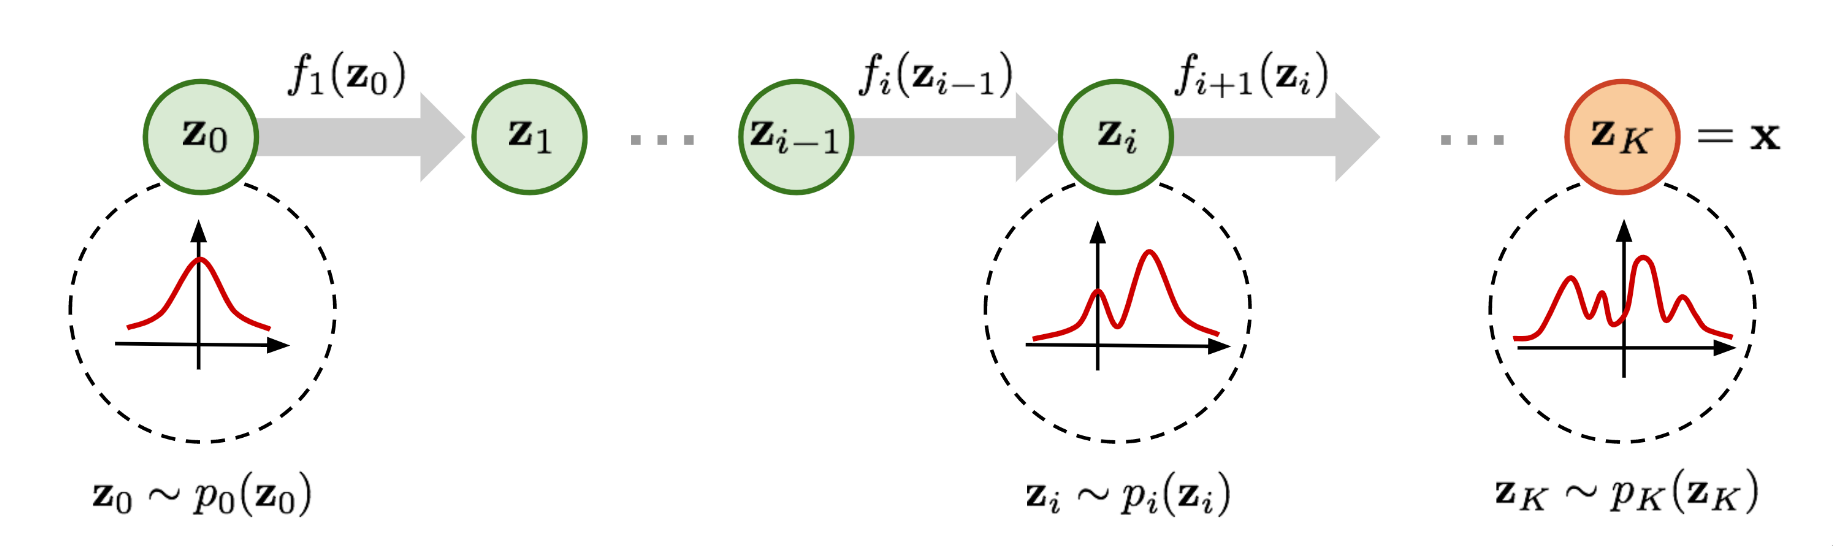
\includegraphics[width=1.0\linewidth]{figures/normalizing-flow.png}
    \end{figure}
    \onslide<2->{
    \begin{center}
        \emph{How do we learn such a sequence of functions \( f_i \)?}
    \end{center}
    }
\end{frame}
\begin{frame}
    Given \textbf{invertible}, \textbf{smooth both ways} function \( T : \mathbb{R}^d \to \mathbb{R}^d \).
    \begin{blackblock}
    \emph{Change of variables theorem}
    \begin{align*}
        \int_{\mathbb{R}^d} p_{0}(\mathbf{x}) \mathrm{d}\mathbf{x} = \int_{\mathbb{R}^d} p_0(T^{-1}(\mathbf{y})) \left| \det \frac{\partial T}{\partial y} \right|^{-1}  \mathrm{d} \mathbf{y}
    .\end{align*}
    \end{blackblock}
    \begin{figure}
        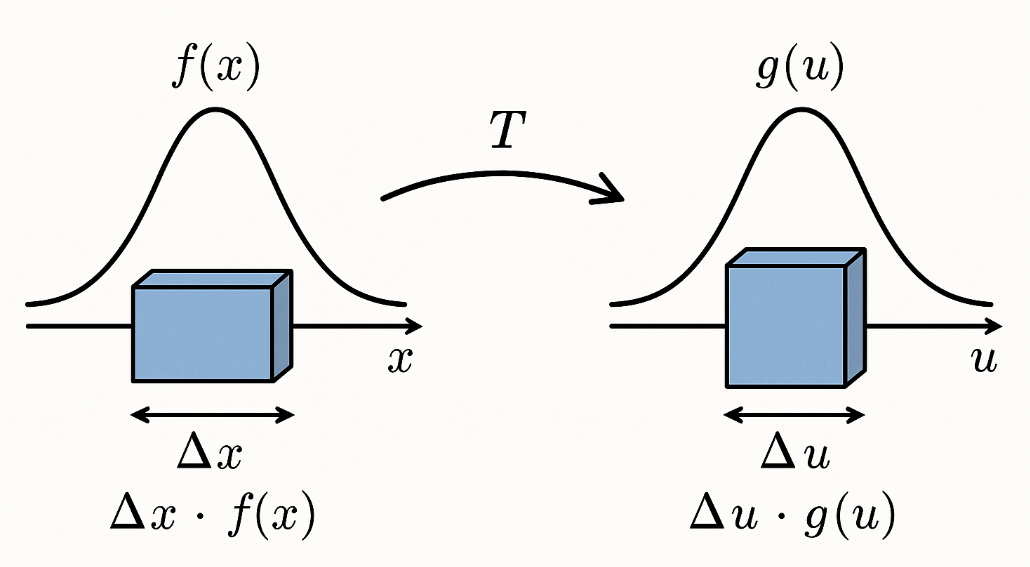
\includegraphics[width=0.5\linewidth]{figures/COVT.png}
    \end{figure}
    \( \Rightarrow \) Density of \( f_{1}(\mathbf{z}_0) = p_{0}(\mathbf{z}_0) \left| \det \frac{\partial f_{1}}{\partial \mathbf{z}} \right|^{-1}  \) \\
    \( \Rightarrow \) \( \log p_K(\mathbf{z}_k) = \log p_{0}(\mathbf{z}_0) - \sum_{k = 1}^{K} \left| \det \frac{\partial f_{k}}{\partial \mathbf{z}_{k - 1}} \right|^{-1}  \)
\end{frame}
\begin{frame}
    \begin{minipage}{0.7\linewidth}
    \begin{blackblock}
        \( \log p_K(\mathbf{z}_k) = \log p_{0}(\mathbf{z}_0) - \sum_{k = 1}^{K} \left| \det \frac{\partial f_{k}}{\partial \mathbf{z}_{k-1}} \right|^{-1}  \)
    \end{blackblock}
    \end{minipage}
    \begin{enumerate}
        \item Given \( \mathbf{x}^{(i)} \) from dataset, compute \( \mathbf{x}^{(i)}_0 = (f_{K} \circ \cdots \circ f_{1})^{-1}(\mathbf{x}^{(i)}) \)
        \item<2-> Maximize log-likelihood
            \begin{align*}
                \max_{\theta} \left[\log p_{0}(\mathbf{x}_{0}^{(i)}(\theta)) - \sum_{k = 1}^{K} \left| \det \frac{\partial f_{k}(\theta)}{\partial \mathbf{x}^{(i)}_{k - 1}} \right|^{-1}\right] 
    \tikz[remember picture,overlay] \coordinate (eqpos);
            .\end{align*}
    \end{enumerate}
    \onslide<3->{
    \begin{tikzpicture}[remember picture,overlay]
    % Draw the box around the equation coordinate
    \draw[red, dashed, thick]
        ([xshift=-8em,yshift=-3.5ex]eqpos) rectangle ([xshift=-.5em,yshift=5ex]eqpos);

    % Draw an arrow pointing to the box with a label
    \draw[<-, dashed, thick, red]
        ([xshift=-.5em,yshift=5ex]eqpos) -- ++(1,.5)
        node[right, red] {$O(LD^3)$};
    \end{tikzpicture}
    }
    \vspace*{-0.7cm}
    \onslide<4->{
    \begin{redblock}
        \color{red} Need to pick \textbf{simple} transformations i.e.
        \begin{align*}
            f(\mathbf{z}) = \mathbf{z} + \mathbf{u}h(\mathbf{w}^{\top} \mathbf{z} + b)
        .\end{align*}
        Require \textbf{very large} \( K \) to represent complex distributions.
    \end{redblock}
    }
    \onslide<5->{
    \emph{Why not take \( K \to \infty\)...}
    }
    \vspace*{-.5cm}
\end{frame}
\begin{frame}{Neural Ordinary Differential Equations \cite{chenNeuralOrdinaryDifferential}}
    \vspace*{-.25cm}
    \begin{columns}
        \begin{column}{0.59\linewidth}
        Replace \( \mathbf{z}_{t + 1} = f_t(\mathbf{z}_t) \) with the \textbf{ODE} 
        \begin{align*}
            \frac{\mathrm{d}\mathbf{z}}{\mathrm{d}t} = f_t(\mathbf{z}_t)
        .\end{align*}
        \end{column}
        \begin{column}{0.4\linewidth}
            \vspace{-.25cm}
            \begin{blackblock}
                \footnotesize
                \textbf{Remark.} \emph{Instantaneous COV}
                \[ \frac{\partial \log p_t(\mathbf{z}_t)}{\partial t} = -\text{tr}\left(\frac{df}{d\mathbf{z}_t}\right) \]
            \end{blackblock}
        \end{column}
    \end{columns}
    \vspace{.5cm}
    \onslide<2->{
    {\color{red}
    Given \( \mathbf{x}^{(i)} \) from dataset, now must compute \( \mathbf{x}^{(i)}_0 = \int_{1}^{0} f^{-1}_t (\mathbf{x}^{(i)}_t) \mathrm{d}t \)
    \begin{itemize}
        \color{red}
        \item Requires \textbf{exact} ODE solve for unbiased gradient.
    \end{itemize}
    }
    \begin{figure}
        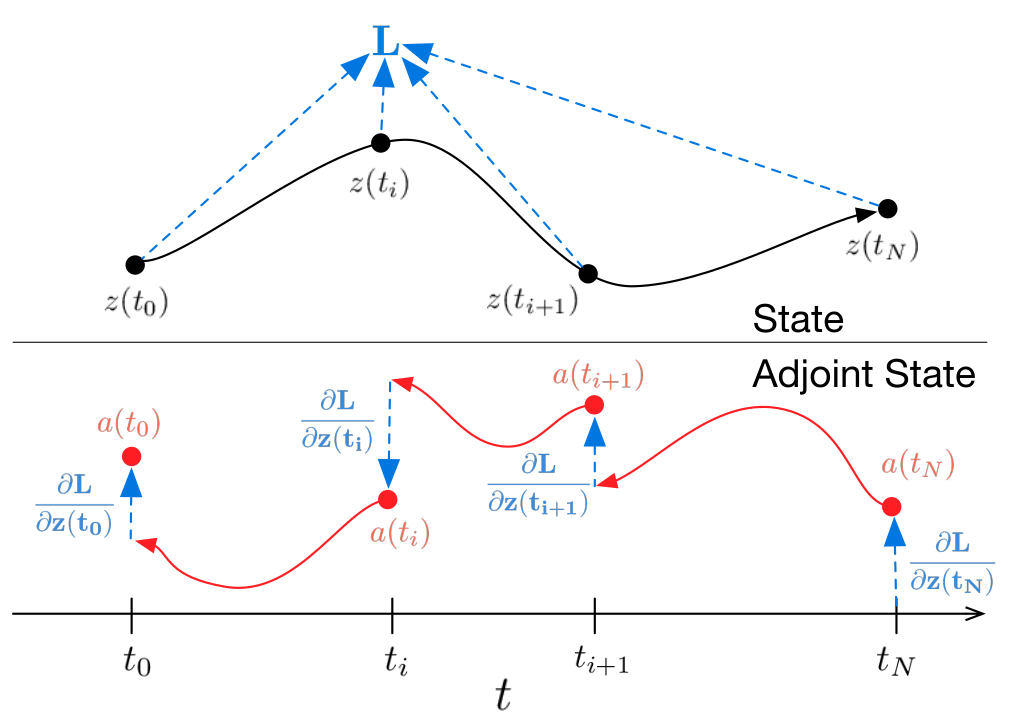
\includegraphics[width=0.5\linewidth]{figures/ode-backprop.png}
    \end{figure}
    }
    \onslide<3->{
    \emph{Can we learn \( f_t \) without backprop through an ODE?}
    }
\end{frame}
\begin{frame}{Flow Matching for Generative Modeling \cite{lipmanFlowMatchingGenerative2023}}
    \begin{blackblock}
    \textbf{Disclaimer:} \( f_t \) will now often be referred to as the \emph{flow}.
    \end{blackblock}
    \textbf{Book keeping.} We say the \emph{flow} \( f_t \) \emph{generates} a probability path \( p_t \) if \( X_t = f_t(X_{0}) \sim p_t \). Equivalently,
    \begin{align*}
        p_t(x) = [f_{t\sharp}p_0](x) \triangleq  p_0(f_t^{-1}(y)) \left|\det \partial_y f_t^{-1}(y)\right|
    .\end{align*}
    \begin{figure}
        \centering
        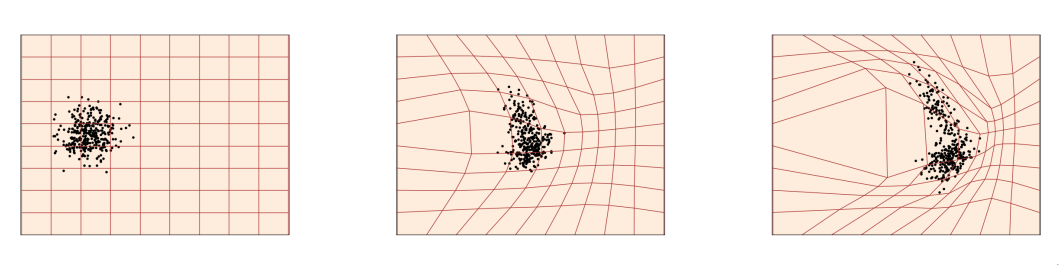
\includegraphics[width=\linewidth]{figures/flow-vis.png}
    \end{figure}
\end{frame}
\begin{frame}
    \begin{blackblock}
    \textbf{Key Idea:} Do \textbf{not} learn the \emph{flow} \( f_t \), learn the \textbf{velocity} of the flow.
    \end{blackblock}
\textbf{Def.} This velocity is a \emph{vector field} \( u_t : \mathbb{R}^d \to \mathbb{R}^d \), such that
\begin{align*}
    \frac{\mathrm{d}f_t(\mathbf{x})}{\mathrm{d}t} = u_t(f_t(\mathbf{x}))
.\end{align*}
\onslide<2->{
To sample, solve ODE at \textbf{sample time} i.e.
\begin{align*}
    f_{t + \Delta t}(\mathbf{x}) \approx f_t(\mathbf{x}) + \Delta t \cdot u_t(f_t(\mathbf{x})) \tag*{(Euler method)}
\end{align*}
By uniqueness of ODE, (vector field \(u_t\)) \( \leftrightarrow \) (flow \( f_t \)). \\
\vskip 5pt
\begin{figure}
    \centering
    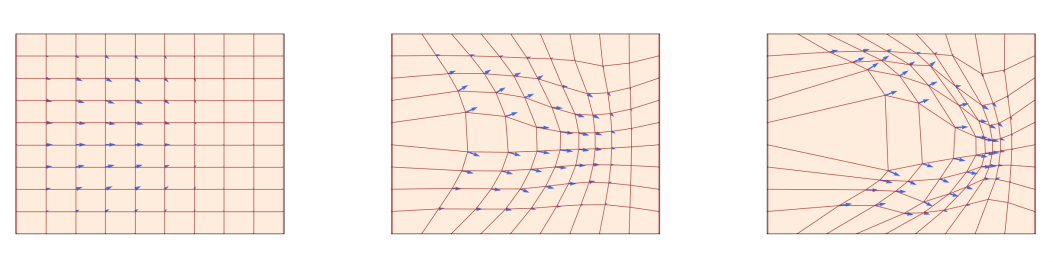
\includegraphics[width=\linewidth]{figures/vector-vis.png}
\end{figure}
}
\end{frame}
\begin{frame}
    \textbf{Def.} A \emph{vector field} \( u_t \) \emph{generates} a probability path \( p_t \) if its corresponding flow \( f_t \) \emph{generates} \( p_t \). \\
    \vskip 5pt
    \textbf{Thm.} A \emph{vector field} \( u_t \) \emph{generates} a probability path \( p_t \) if and only if it satisfies the \emph{continuity equation}.
    \begin{blackblock}
    \textbf{Continuity Equation.}
    \[ \frac{\mathrm{d}}{\mathrm{d}t}p_t(x) + \mathrm{div}(p_t u_t)(x) = 0, \]
    where $\text{div}(v)(x) = \sum_{i=1}^{d} \partial_{x^{i}} v^{i}(x)$, and $v(x) = (v^{1}(x), \ldots, v^{d}(x))$.
    \end{blackblock}
    \begin{figure}
        \centering
        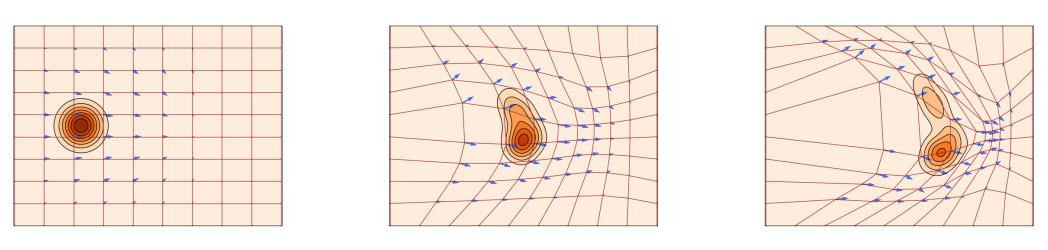
\includegraphics[width=\linewidth]{figures/density-vis.png}
    \end{figure}
\end{frame}
\begin{frame}
    \begin{blackblock}
    \textbf{Continuity Equation.}
    \[ \frac{\mathrm{d}}{\mathrm{d}t}p_t(x) + \mathrm{div}(p_t u_t)(x) = 0, \]

    where $\text{div}(v)(x) = \sum_{i=1}^{d} \partial_{x^{i}} v^{i}(x)$, and $v(x) = (v^{1}(x), \ldots, v^{d}(x))$.
    \end{blackblock}
    \textbf{Proof: (If people care)}
    \begin{align*}
        \frac{d}{dt}\mathbb{E}f(X_t) &= \frac{d}{dt}\int_{\mathbb{R}^d} f(x)p_t(x)dx = \int_{\mathbb{R}^d} f(x)\partial_t p_t(x)dx, \\
     \mathbb{E}\frac{d}{dt}f(X_t) &= \int_{\mathbb{R}^d} \left(\nabla f(x_t)\cdot v_t(x_t)\right) p_t(x_t)dx_t \\  
                                  &= 0 - \int_{\mathbb{R}^d} f(x_t)\text{div}(v_t(x_t)p_t(x_t))dx_t \tag*{(IBP)}\\ 
                                  &= \int_{\mathbb{R}^d} -f(x)\text{div}(v_t(x)p_t(x))dx.
    .\end{align*}
    The result follows from fundamental lemma of calculus of variations.

\end{frame}

\section{Flow Matching}
\begin{frame}
    \begin{center}
        \emph{How do we actually learn the vector field \( u_t \)?}
    \end{center}
\end{frame}
\begin{frame}
    \begin{blackblock}
        \textbf{Flow Model Loss}
        \[ \mathcal{L}_{\text{\tiny FM}}(\theta) = \mathbb{E}_{t, p_t(x)} \|v_{t}(x; \theta) - u_t(x)\|^2 \]
    \end{blackblock}
    \begin{itemize}
        \item \( p_t : \mathcal{X} \to [0, 1] \): probability density path.
        \item \( u_t : \mathbb{R}^d \to \mathbb{R}^d \): vector field that \emph{generates} \( p_t \).
    \end{itemize}
    \vspace*{.5cm}
    \onslide<2->{
    \begin{redblock}
        \color{red}
        \textbf{Intractable.}
        \begin{enumerate}
            \color{red}
            \item How to choose \( p_t \)?
            \item<3-> Given \( p_t \) need to solve continuity equation for \( u_t \), which is a \textbf{PDE} likely without close-form.
        \end{enumerate}
    \end{redblock}
    }
\end{frame}

\begin{frame}
    \begin{blackblock}
    \textbf{Key Idea:} \emph{Given the endpoint \( X_{1} \), we can easily construct a path between \( X \) and \( X_{1} \).}
    \end{blackblock}
    \textbf{Ex:} \emph{Consider} \[ f_t(x \mid x_{1}) = tx_{1} + (1 - (1 - \sigma_{\mathrm{min}})t)x \]
    \vskip 3pt
    \begin{columns}
        \begin{column}{0.49\linewidth}
        \begin{figure}
            \centering
            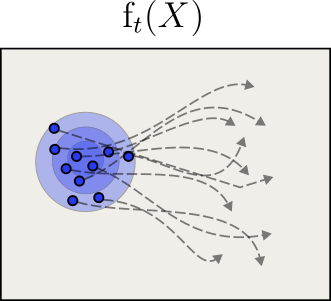
\includegraphics[width=0.8\linewidth]{figures/marginal-path.png}
        \end{figure}
        \end{column}
        \begin{column}{0.49\linewidth}
        \begin{figure}
            \centering
            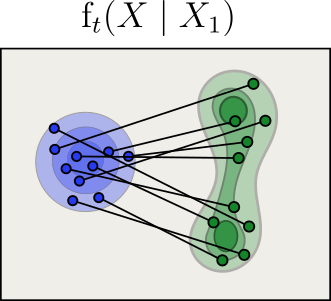
\includegraphics[width=0.8\linewidth]{figures/conditional-path.png}
        \end{figure}
        \end{column}
    \end{columns}
\end{frame}
\begin{frame}
    \begin{center}
        \emph{What does the conditional flow being nice have to do with our problem?}
    \end{center}
\end{frame}
\begin{frame}
    \textbf{Idea 1:} Given target data distribution \( q \), approximate \( q \) by marginalizing ``nice'' conditionals by \( q \) i.e.
    \begin{align*}
        p_t(\mathbf{x}) = \int p_t(\mathbf{x} \mid \mathbf{x}_{1}) q(\mathbf{x}_{1}) \mathrm{d}\mathbf{x}_{1} \tag*{(Marginal Density)}
    .\end{align*}
    For \( p_{1}(\mathbf{x} \mid \mathbf{x}_{1}) \sim N(x_{1}, \sigma_{1}) \), with \( \sigma_{1} \ll 1 \), \( p_{1}(\mathbf{x}) \approx q(\mathbf{x}) \). \\
    \vskip 5pt
    \onslide<2->{
    \textbf{Idea 2:} Use this to define an approximate vector field
    \begin{align*}
        u_t(\mathbf{x}) = \int u_t(\mathbf{x} \mid \mathbf{x}_1) \frac{p_t(\mathbf{x} \mid \mathbf{x}_1)q(\mathbf{x}_1)}{p_t(\mathbf{x})}\mathrm{d}\mathbf{x}_1 \tag*{(Marginal Vector Field)}
    .\end{align*}
    Here, \( u_t(\mathbf{x} \mid \mathbf{x}_1) \) is the conditional vector field that generates \( p_t(\mathbf{x} \mid \mathbf{x}_1) \).
    }
    \onslide<3->{
        \begin{blackblock}
            \textbf{Thm.} \emph{The marginal vector field \( u_t \) generates the marginal probability path \( p_t \).} (Check continuity equation)
        \end{blackblock}
    }
    
\end{frame}

\begin{frame}
    \begin{blackblock}
    \textbf{Conditional Flow Model Loss} \[ \mathcal{L}_{\text{\tiny CFM}}(\theta) = \mathbb{E}_{t, q(x_{1}), p_t(x \mid x_{1})} \|v_{t}(x; \theta) - u_t(x \mid x_{1})\|^2 \]
    \end{blackblock}
    \onslide<2->{
    \begin{blackblock}
        \textbf{Thm.} \emph{Up to a constant independent of \( \theta \), \( \mathcal{L}_{\text{\tiny FM}}(\theta ) =  \mathcal{L}_{\text{\tiny CFM}}(\theta )\). In particular, \( \nabla \mathcal{L}_{\text{\tiny FM}}(\theta ) =  \nabla \mathcal{L}_{\text{\tiny CFM}}(\theta )\)}. 
    \end{blackblock}
    \begin{columns}
        \begin{column}{0.28\linewidth}
        \begin{figure}
            \centering
            \textbf{Batch} \( i \)
            \vskip 2pt
            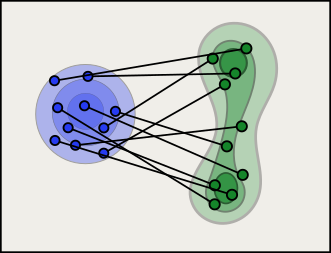
\includegraphics[width=\linewidth]{figures/batch-1.png}
        \end{figure}
        \end{column}
        \begin{column}{0.28\linewidth}
        \begin{figure}
            \centering
            \textbf{Batch} \( j \)
            \vskip 2pt
            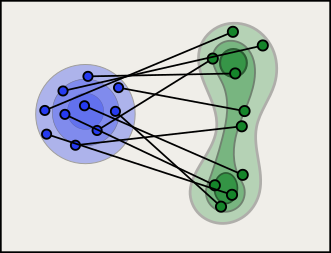
\includegraphics[width=\linewidth]{figures/batch-2.png}
        \end{figure}
        \end{column}
        \begin{column}{0.28\linewidth}
        \begin{figure}
            \centering
            \( \mathbb{E}[\textbf{Batch}] \)
            \vskip 2pt
            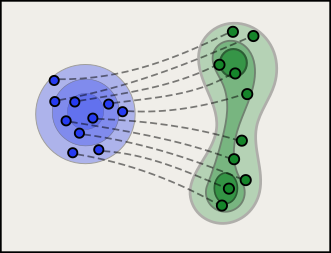
\includegraphics[width=\linewidth]{figures/avg-interpolation.png}
        \end{figure}
        \end{column}
    \end{columns}
    }
\end{frame}
\begin{frame}
    \begin{center}
        \emph{How do we actually use this?}
    \end{center}
\end{frame}

\begin{frame}{Example: Optimal Transport}
    \only<1-3>{
    For \( f_t(x) = \mu_t(x_{1}) + x \sigma_t(x_{1}) \), we consider
    \begin{align*}
        \mu_t = tx_{1}, \quad \sigma_t(x) = 1 - (1 - \sigma_{\min})t
    ,\end{align*}
    such that
    }
    \only<2-3>{
        \begin{align*}
            f_t^{-1}(x) = \frac{x - tx_{1}}{1 - (1-\sigma_{\min})t}, \quad \frac{\mathrm{d}}{\mathrm{d}t} f_t(x) = x_{1} - (1 - \sigma_{\min})x
        .\end{align*}
    }
    \only<3->{
    Recall
    \begin{align*}
        \frac{\mathrm{d}}{\mathrm{d}t} f_t(x) = u(f_t(x) \mid x_{1}) \implies u(x \mid x_{1}) = \frac{\mathrm{d}}{\mathrm{d}t} f_t(f_t^{-1}(x))
    .\end{align*}
    }
    \only<4->{
        Thus,
        \begin{align*}
            &u_t(x \mid x_{1}) = \frac{x_{1} - (1 - \sigma_{\min})x}{1 - (1 - \sigma_{\min})t}
        .\end{align*}
    }
    \only<5->{
        \begin{blackblock}
            \centering
            $\mathcal{L}_{\text{\tiny CFM}}(\theta) = \mathbb{E}_{t, q(x_{1}), p_t(x \mid x_{1})} \left\|v_{t}(x; \theta) - \frac{x_{1} - (1 - \sigma_{\min})x}{1 - (1 - \sigma_{\min})t}\right\|^2$
        \end{blackblock}
    }
\end{frame}

\begin{frame}{Diffusion Meets Flow Matching: Two Sides of the Same Coin \cite{gaoDiffusionMeetsFlow2024}}
    Recall that instead of an ODE, in diffusion, we have a \textbf{SDE}
    \begin{align*}
        \mathrm{d}\mathbf{x}_t = f_t(\mathbf{x}_t)\mathrm{d}t + \sigma(\mathbf{x}_t) \mathrm{d}B_t
    .\end{align*}
    However, for \emph{OU} process, we can actually absorb Brownian motion term and get vector field
    \begin{align*}
        u_t(\mathbf{x}_t) = -(\mathbf{x}_t + \nabla \ln p_t(\mathbf{x}_t))
    .\end{align*}
    Similarly, learning the score function \( \nabla \ln p_t(\mathbf{x}_t) \) can be rewritten as the flow matching objective for certain choices of \( p_t \) see \cite{lipmanFlowMatchingGuide2024a}.
\end{frame}

\begin{frame}{Why Flows?}
    \begin{blackblock}
        \textbf{Anecdotally.}
        \begin{itemize}
            \item{\footnotesize \emph{The OT path’s conditional
                vector field has constant direction in time and is arguably simpler to fit with a parametric model. \cite{lipmanFlowMatchingGenerative2023}}}
            \item{\footnotesize \emph{The deterministic
                nature of ODEs equips flow-matching methods with simpler learning objectives and faster inference speed \cite{zhengIntentionConditionedFlowOccupancy2025}}}
        \end{itemize}
    \end{blackblock}
    \vspace*{.5cm}
\begin{figure}
    \hspace*{-.5cm}
    \begin{minipage}{0.50\linewidth}
    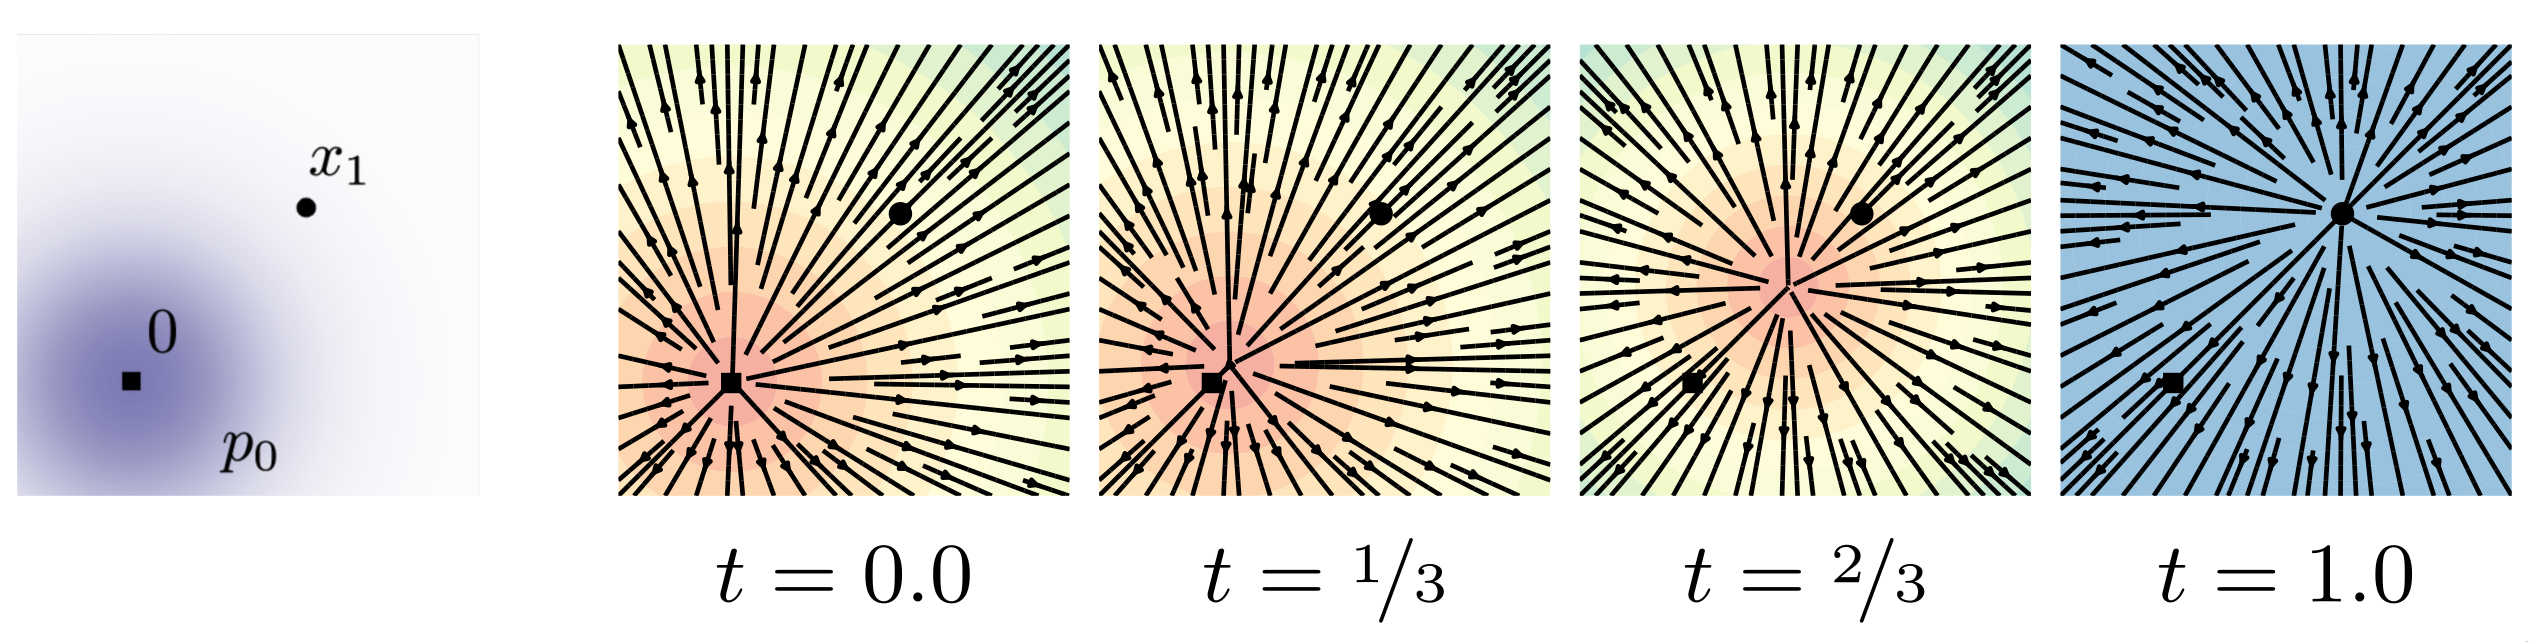
\includegraphics[width=1.2\linewidth]{figures/conditional-score.png}
    \hspace*{2.5cm}
    {\footnotesize Conditional score}
    \end{minipage}
    \hspace*{1cm}
    \begin{minipage}{0.39\linewidth}
    \centering
    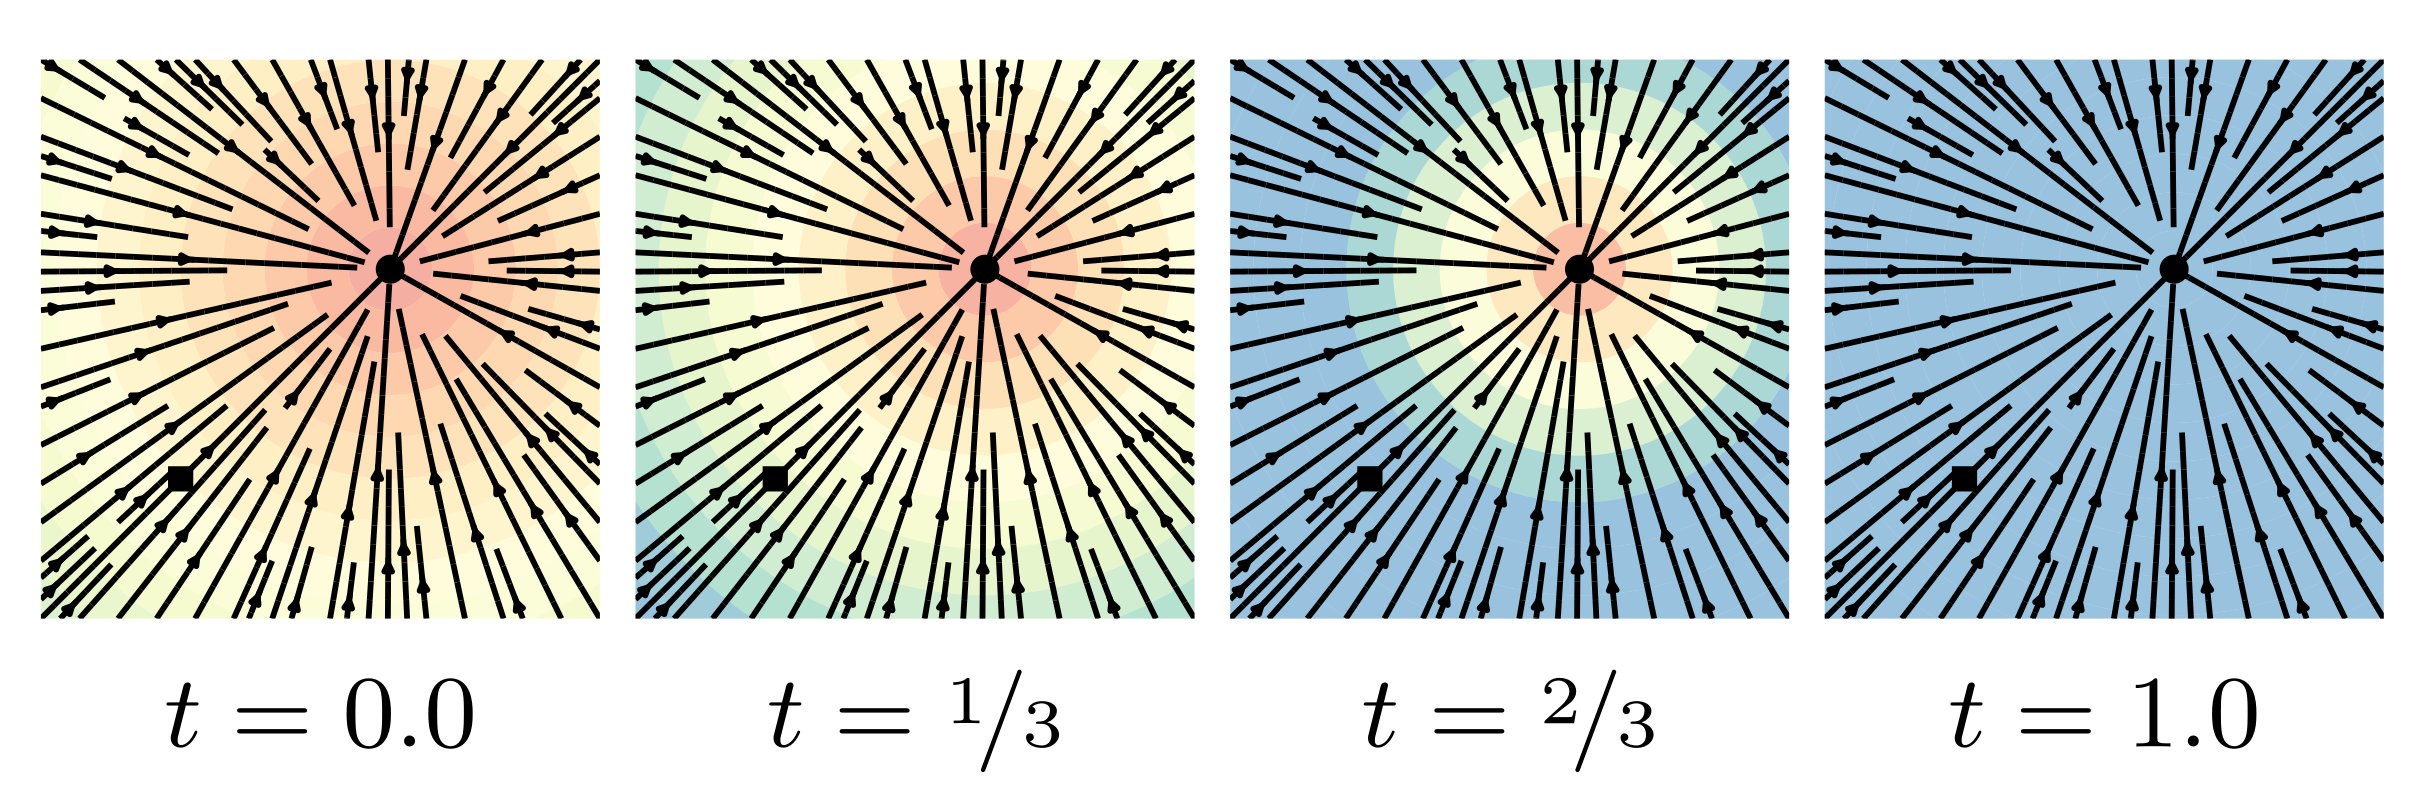
\includegraphics[width=1.2\linewidth]{figures/conditional-vector-field.png}
    {\footnotesize Conditional vector field}
    \end{minipage}
\end{figure}
\end{frame}

\section{Application to Reinforcement Learning}
\begin{frame}{Q learning is not yet scalable \cite{parkQlearningNotScalable2025}}
    \textbf{Long horizon problems are hard.}
    \begin{align*}
\mathbb{E}_{(s,a,r,s')\sim \mathcal{D}}\bigg[\Big(Q_\theta(s,a)-\underbrace{\big(r+\gamma \max_{a'}Q_{\bar{\theta}}(s',a')\big)}_{\texttt{Biased}}\Big)^2\bigg]
    .\end{align*}
    \begin{columns}
        \hspace*{-1cm}
        \begin{column}{0.3\linewidth}
        \begin{figure}
            \centering
            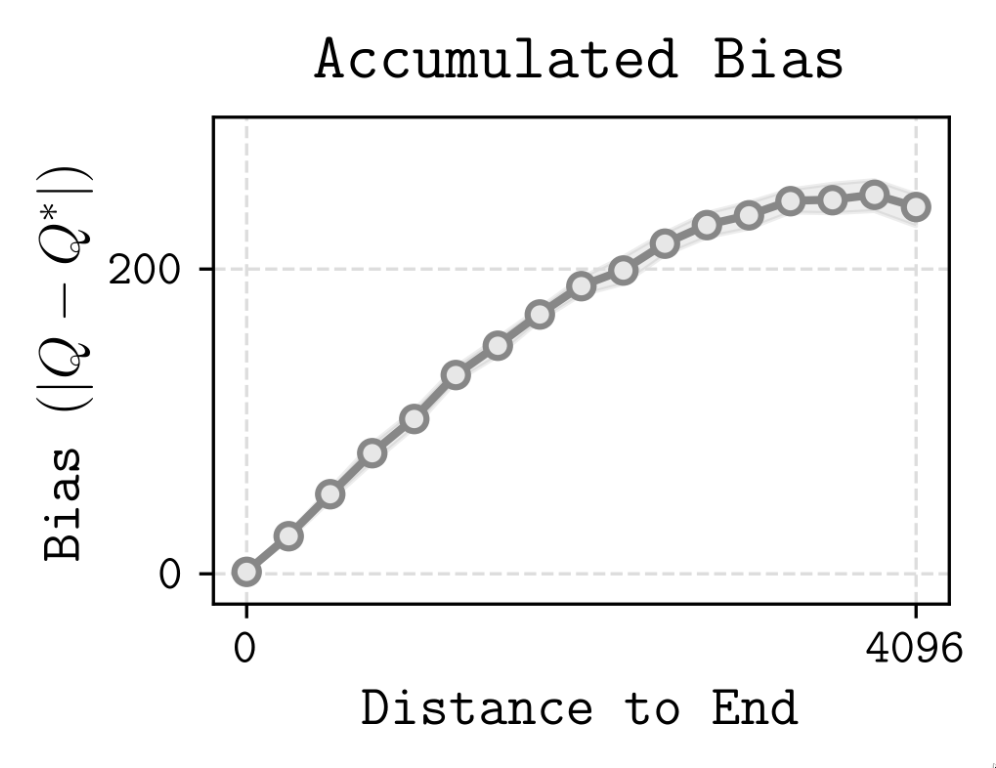
\includegraphics[width=\linewidth]{figures/bias_accumulation.png}
        \end{figure}
       \end{column} 
       \hspace*{-1cm}
       \begin{column}{0.69\linewidth}
        \vspace*{-.5cm}
        \begin{figure}
            \centering
            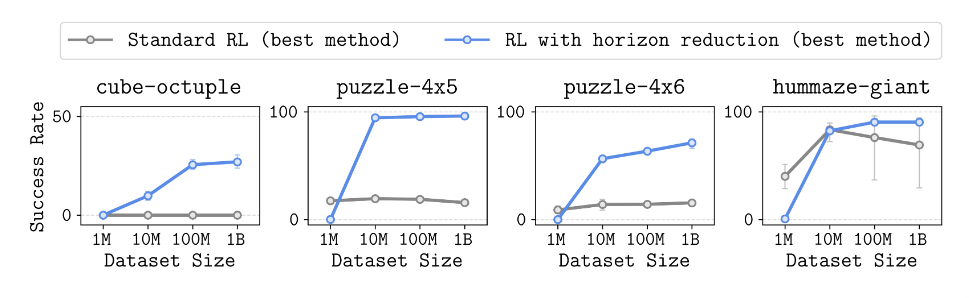
\includegraphics[width=1.1\linewidth]{figures/horizon-reduction.png}
        \end{figure}
       \end{column}
    \end{columns}
\end{frame}
\begin{frame}{Temporal Difference Flows \cite{farebrotherTemporalDifferenceFlows2025}}
    \begin{blackblock}
        \textbf{Idea:} Apply flow matching to learn the \emph{successor measure} of an MDP.
    \end{blackblock}
    \textbf{Def.} We define the \emph{successor measure} as
\[ m^{\pi}(\mathsf{X} \mid s, a) = (1 - \gamma) \sum_{k=0}^{\infty} \gamma^{k} \Pr(S_{k+1} \in \mathsf{X} \mid S_{0} = s, A_{0} = a, \pi), \]
\textbf{Recall.} The \emph{successor measure} is the unique fix point to the \emph{Bellman} equation
\begin{align*}
 m^{\pi}(\cdot \mid s, a) &= (\mathcal{T}^{\pi} m^{\pi}) (\cdot \mid s, a) \\
                          &:= (1 - \gamma)P(\cdot \mid s, a) + \gamma (P^{\pi} m^{\pi}) (\cdot \mid s, a)
,\end{align*}
where
\[ (P^{\pi}m) (\mathrm{d}x \mid s, a) = \int_{s'} P(\mathrm{d}s' \mid s, a) m(\mathrm{d}x \mid s', \pi(s')). \]
\end{frame}
\begin{frame}
    The most straightforward idea is to just substitute \( m^{\pi} \) for \( q \) in flow matching i.e.
\[ \mathcal{L}_{\text{MC-CFM}}(\theta) = \mathbb{E}_{\rho, t, Z, X_t} \Big[ \big\| \tilde{v}_t(X_t \mid S, A; \theta) - u_{t}(X_t \mid Z) \big\|^2 \Big], \] where $Z = X_1 \sim m^{\pi}(\cdot \mid S, A), X_t \sim p_{t}(\cdot \mid Z).$ \\
\vskip 5pt
Here we just use the optimal transport conditional vector field and corresponding probability density path. \\
\vskip 5pt
\onslide<2->{
{\color{red} This requires direct access to samples from \( m^{\pi} \).} \\
\vskip 5pt
\emph{Can we learn from offline one-step transitions \( (S, A, S') \)?} \\
\vskip 5pt
}
\onslide<3->{
\begin{blackblock}
Leverage \textbf{recursive} structure of Bellman equation i.e.
\begin{gather*}
    X_{0} \sim p_{0} \\
    Z = X_1 \sim (1 - \gamma)\delta_{S'} + \gamma \delta_{\tilde{f}_1(X_0 \mid S', \pi(S'))} \tag*{(TD-CFM)}
.\end{gather*}
\end{blackblock}
}
    \end{frame}
    \begin{frame}
    \begin{blackblock}
    Leverage \textbf{recursive} structure of Bellman equation i.e.
    \begin{gather*}
        X_{0} \sim p_{0} \\
        Z = X_1 \sim (1 - \gamma)\delta_{S'} + \gamma \delta_{\tilde{f}_1(X_0 \mid S', \pi(S'))}
    .\end{gather*}
    \end{blackblock}
    \begin{itemize}
        \item With probability \( (1 - \gamma) \), \( X_{1} = S' \)
        \item With probability \( \gamma \), sample from \( \tilde{m}^{\pi} \) by integrating \( \tilde{f}_t \).
    \end{itemize}
    \vspace*{1cm}
        \begin{center}
            \emph{Can we do better?}
        \end{center}
    \end{frame}
    
    \begin{frame}
    \textbf{Lemma}. Let $v_t^1$ and $v_t^2$ be vector fields that generate the probability paths $p_t^1$ and $p_t^2$, respectively. Then, for any $\gamma \in [0, 1]$, the mixture probability path $p_t = (1 - \gamma)p_t^1 + \gamma p_t^2$ is generated by the vector field.
\[ v_t := \frac{(1-\gamma)p_t^1v_t^1 + \gamma p_t^2v_t^2}{(1-\gamma)p_t^1 + \gamma p_t^2}. \]
\onslide<2->{
\textbf{Remember} The \emph{successor measure} is the unique fix point to the \emph{Bellman} equation
\begin{align*}
 m^{\pi}(\cdot \mid s, a) &= (1 - \gamma)P(\cdot \mid s, a) + \gamma (P^{\pi} m^{\pi}) (\cdot \mid s, a)
,\end{align*}
where
\[ (P^{\pi}m) (\mathrm{d}x \mid s, a) = \int_{s'} P(\mathrm{d}s' \mid s, a) m(\mathrm{d}x \mid s', \pi(s')). \]
}
\onslide<3->{
\begin{blackblock}
    \textbf{Idea:} Learn \( v_t \) for \( p_t^1 = P(\cdot \mid S, A) \), \( p_t^2 = (P^{\pi} m)(\cdot \mid S, A) \)
\end{blackblock}
}
    \end{frame}
\begin{frame}
    \textbf{Lemma.} Let $v_t^1$ and $v_t^2$ be vector fields that generate the probability paths $p_t^1$ and $p_t^2$, respectively. For $\gamma \in [0,1]$, the vector field $v_t = \frac{(1-\gamma)p_t^1v_t^1 + \gamma p_t^2v_t^2}{(1-\gamma)p_t^1 + \gamma p_t^2}$ satisfies
    \begin{align*}
        v_t = \underset{v: \mathbb{R}^d \to \mathbb{R}^d}{\arg \min} \Big\{ (1 - \gamma) &\mathbb{E}_{x_t \sim p_t^1} \left[ ||v_t(x_t) - v_t^1(x_t)||^2 \right] \\ &+ \gamma \mathbb{E}_{x_t \sim p_t^2} \left[ ||v_t(x_t) - v_t^2(x_t)||^2 \right] \Big\}
    .\end{align*}
    \onslide<2->{
        \vspace*{-.25cm}
    \begin{blackblock}
        \textbf{Substitute.}
    \begin{align*}
        v_t = \underset{v: \mathbb{R}^d \to \mathbb{R}^d}{\arg \min} \Big\{ (1 - \gamma) &\overbrace{\mathbb{E}_{x_t \sim P} \left[ ||v_t(x_t) - v_t^1(x_t)||^2 \right]}^{\mathcal{L}_{\mathrm{OS}}} \\ &+ \gamma \underbrace{\mathbb{E}_{x_t \sim P^{\pi} m} \left[ ||v_t(x_t) - v_t^2(x_t)||^2 \right]}_{\mathcal{L}_{\mathrm{GHM}}} \Big\}
    .\end{align*}
    \end{blackblock}
}
\onslide<3->{
    \emph{How do we get \( v_t^{1} \) and \( v_t^{2} \)?}
}
\onslide<4->{
    \emph{Conditioning trick} \textbf{separately!}
}
    \end{frame}
    \begin{frame}
        \textbf{Case 1:} \( \mathcal{L}_{\mathrm{OS}} \), \( S' \sim P(\cdot \mid S, A) \)
\[ \vec{v}_t(x \mid s, a) = \int \vec{u}_{t}(x \mid x_1) \frac{\vec{p}_{t}(x \mid x_1) P(\mathrm{d}x_1 \mid s, a)}{\vec{p}_t(x \mid s, a)}, \]
\onslide<2->{
\begin{blackblock}
    \[ \begin{aligned} \mathcal{L}_{COS}(\theta) &= \mathbb{E}_{\rho,t,Z,\vec{X}_t}\Big[\big\|\tilde{v}_t(\vec{X}_t\mid S, A; \theta) - \vec{u}_{t}(\vec{X}_t\mid Z)\big\|^2\Big]\,,\\ &\text{where}\ Z = X_1 \sim P(\cdot\mid S, A),\ \vec{X}_t \sim \vec{p}_{t}(\cdot\mid Z)\, \end{aligned} \]
\end{blackblock}
\begin{itemize}
    \item \( \vec{u}_t(\cdot \mid Z) \), \( \vec{p}_t(\cdot \mid Z) \) can be chosen as in \textbf{traditional} flow matching i.e. OT.
\end{itemize}
}
    \end{frame}
    \begin{frame}
        \textbf{Case 2:} We sample future state
\[ \widehat{v}_t^{(n)}(x \mid s,a) = \int v_t^{(n)}(x \mid s',a') \frac{m_t^{(n)}(x \mid s',a')P(\mathrm{d}s' \mid s,a)}{\widehat{p}_t^{(n)}(x \mid s,a)}, \]
where $\widehat{p}_t^{(n)}(x \mid s, a) = \int m_t^{(n)}(x \mid s', a') P(\text{d}s' \mid s, a)$, and $a' = \pi(s')$. \\
\vskip 5pt
\onslide<2->{
    \textbf{Remark.} They show if \( v_t^{(n)} \) is optimizer of proposed loss then \( v_t^{(n)} \) generates \( m_t^{(n)} \).
}
\onslide<3->{
\begin{blackblock}
    \[ \mathcal{L}_{CGHM}(\theta) = \mathbb{E}_{\rho,t,\widehat{X}_t} \left[ \left\| \tilde{v}_t(\widehat{X}_t \mid S, A; \theta) - \tilde{v}_t^{(n)}(\widehat{X}_t \mid S', \pi(S') \right\|^2 \right], \]where $X_0 \sim p_0$, $S' \sim P(\cdot \mid S, A)$, $\widehat{X}_t = \widetilde{f}_t^{(n)}(X_0 \mid S', \pi(S'))$,
\end{blackblock}
}
    \end{frame}
    \begin{frame}
        Combine the \textbf{objectives}!!
\begin{blackblock}
    \[ \begin{aligned} \mathcal{L}_{COS}(\theta) &= \mathbb{E}_{\rho,t,Z,\vec{X}_t}\Big[\big\|\tilde{v}_t(\vec{X}_t\mid S, A; \theta) - \vec{u}_{t}(\vec{X}_t\mid Z)\big\|^2\Big]\,,\\ &\text{where}\ Z = X_1 \sim P(\cdot\mid S, A),\ \vec{X}_t \sim \vec{p}_{t}(\cdot\mid Z)\, \end{aligned} \]
\end{blackblock}
\begin{center}
    \Large
    \( + \)
\end{center}
\begin{blackblock}
    \[ \mathcal{L}_{CGHM}(\theta) = \mathbb{E}_{\rho,t,\widehat{X}_t} \left[ \left\| \tilde{v}_t(\widehat{X}_t \mid S, A; \theta) - \tilde{v}_t^{(n)}(\widehat{X}_t \mid S', \pi(S') \right\|^2 \right], \]where $X_0 \sim p_0$, $S' \sim P(\cdot \mid S, A)$, $\widehat{X}_t = \widetilde{f}_t^{(n)}(X_0 \mid S', \pi(S'))$,
\end{blackblock}
\vspace*{.5cm}
\[
    \mathcal{L}_{\mathrm{TD}^2\mathrm{-CFM}}(\theta) = (1 - \gamma) \mathcal{L}_{COS}(\theta) + \gamma \mathcal{L}_{CGHM}(\theta) \implies \text{ Lower }\mathbb{E}\nabla \mathcal{L}^2
.\] 
\end{frame}
\begin{frame}
    \begin{columns}
        \begin{column}{0.49\linewidth}
        \begin{figure}
            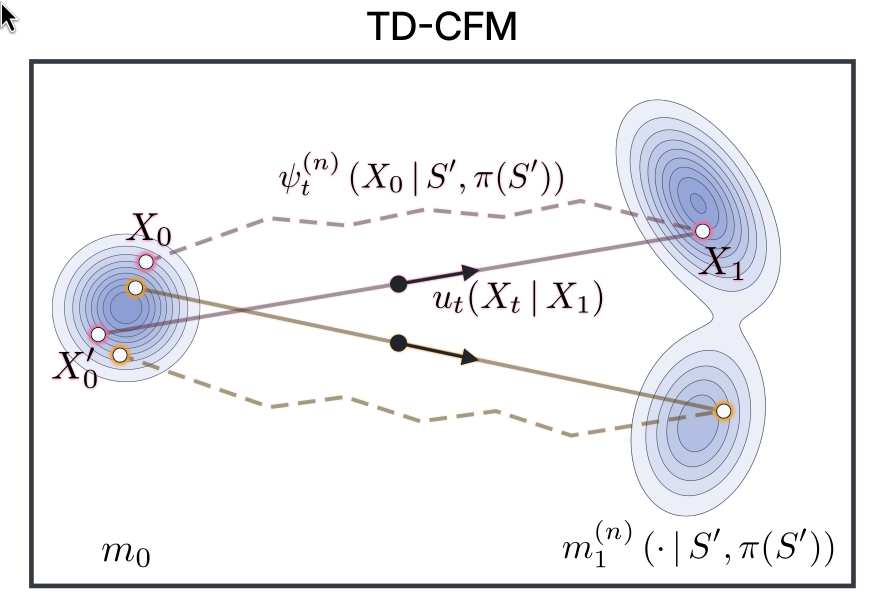
\includegraphics[width=\linewidth]{figures/td-cfm.png}
        \end{figure}
        \end{column}
        \begin{column}{0.49\linewidth}
        \begin{figure}
            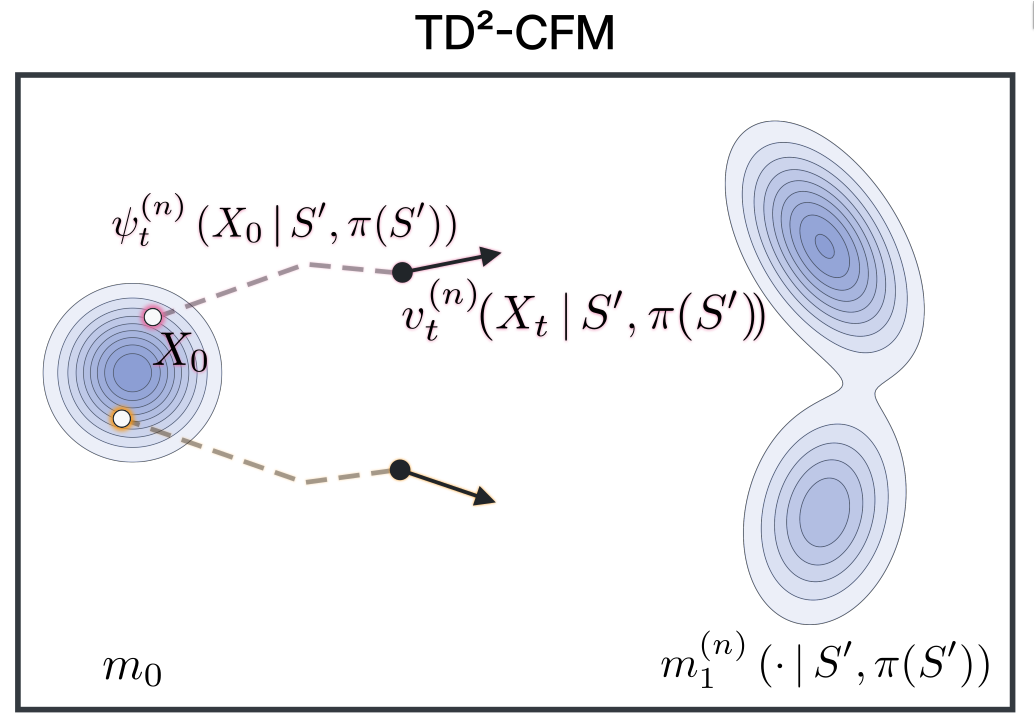
\includegraphics[width=\linewidth]{figures/td2-cfm.png}
        \end{figure}
        \end{column}
    \end{columns}
\end{frame}
\begin{frame}
    \begin{columns}
    \begin{column}{0.6\linewidth}
        \textbf{GPI:}
        \begin{itemize}
        \footnotesize
        \item Train \( \pi_w \) with Forward backward.
        \item Do GPI as $w_t \in \underset{w \sim D(W)}{\arg \max} \underbrace{(1 - \gamma)^{-1} \mathbb{E}_{X \sim m^{\pi_w}(\cdot | s_t, \pi_w(s_t)))}[r(X)]}_{Q^{\pi_w}(s_t, \pi_w(s_t))}.$
        \item Averaged over \( 128 \) samples.
        \end{itemize}
    \end{column}
    \begin{column}{0.4\linewidth}
    \begin{figure}
        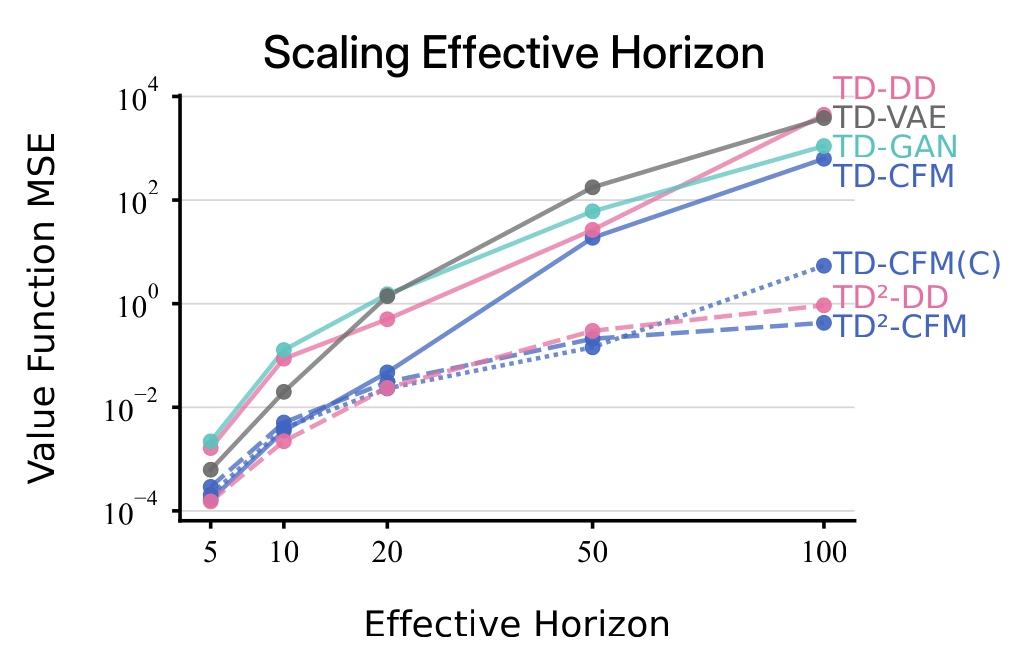
\includegraphics[width=\linewidth]{figures/horizon-td-flow.png}
    \end{figure}
    \end{column}
    \end{columns}
    \begin{figure}
        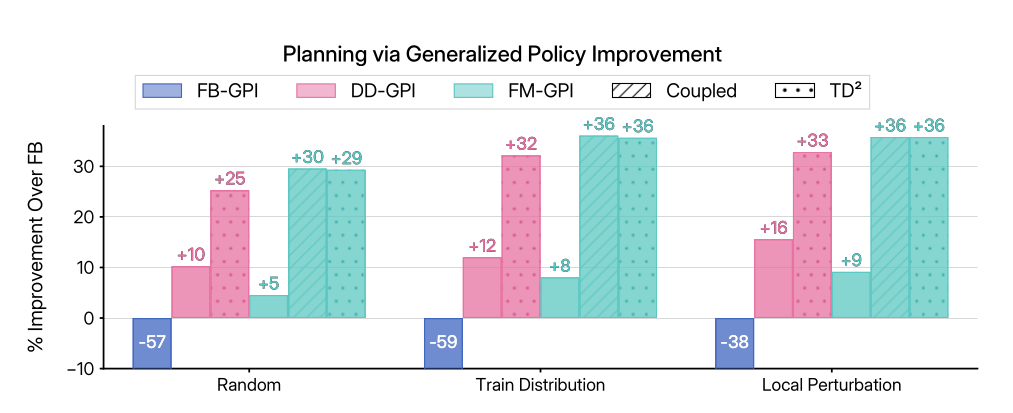
\includegraphics[width=\linewidth]{figures/fm-gpi.png}
    \end{figure}
\end{frame}


\begin{frame}{References}
    \tiny
    \bibliographystyle{alpha}
    \bibliography{references}
\end{frame}

\end{document}
